%SUBSECTION - control
\subsubsection{Simulation results}

In order to predict the behavior of the car to a linear speed reference and angle of tilt (teta), some simulations were necessary. The output of the simulation is the plot of the linear speed of the car, the linear speed of both wheels (left and right) and the position of the car.
In order to plot the position of the car the Cartesian referential is used.\\
For the first simulation, the parameters were: Speed reference= 1m/s and teta=0 rad.\\
\newpage
\begin{figure}[!h]
\centering
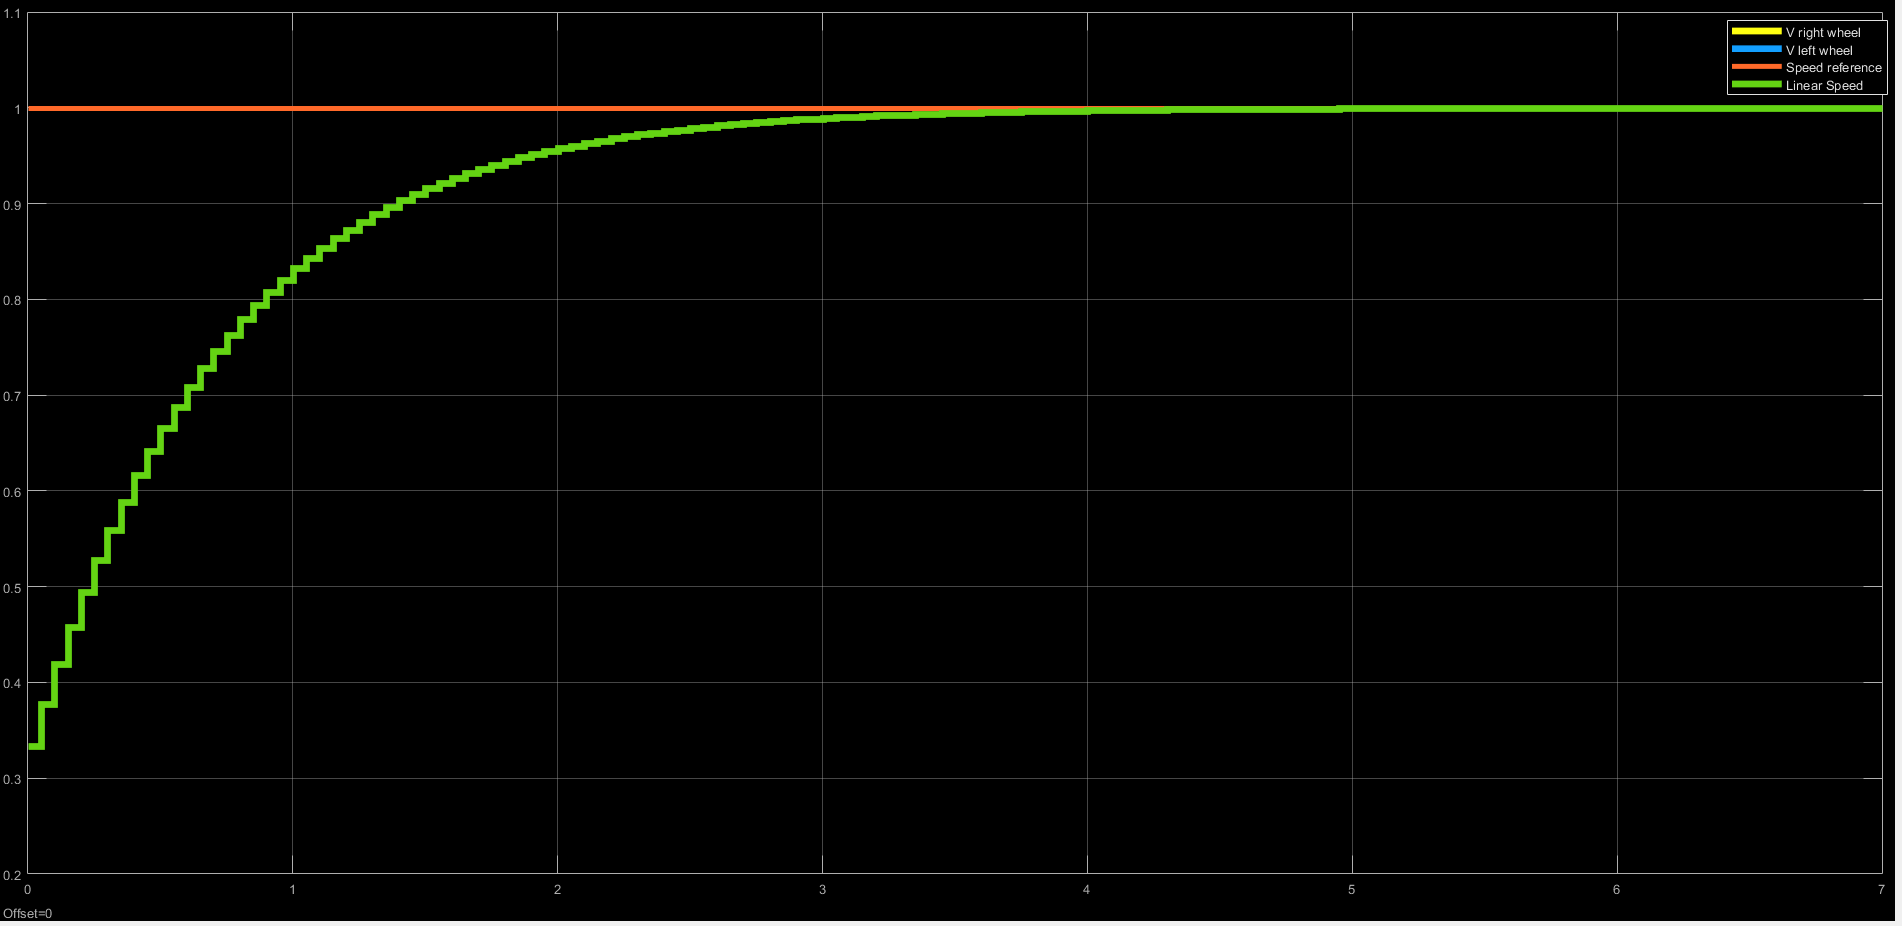
\includegraphics[width=1.0\textwidth]{./img/vel10.PNG}
\caption {\label{fig:sim1 - vel}Linear speed v=1m/s, teta=0rad}
\end{figure}
 As expected, the car linear velocity reached 1m/s. The angle of tilt is equal to 0 which means the car will be moving in a straight line, and as such, both wheels will are moving at the same speed of the car.\\
\newpage
\begin{figure}[!h]
\centering
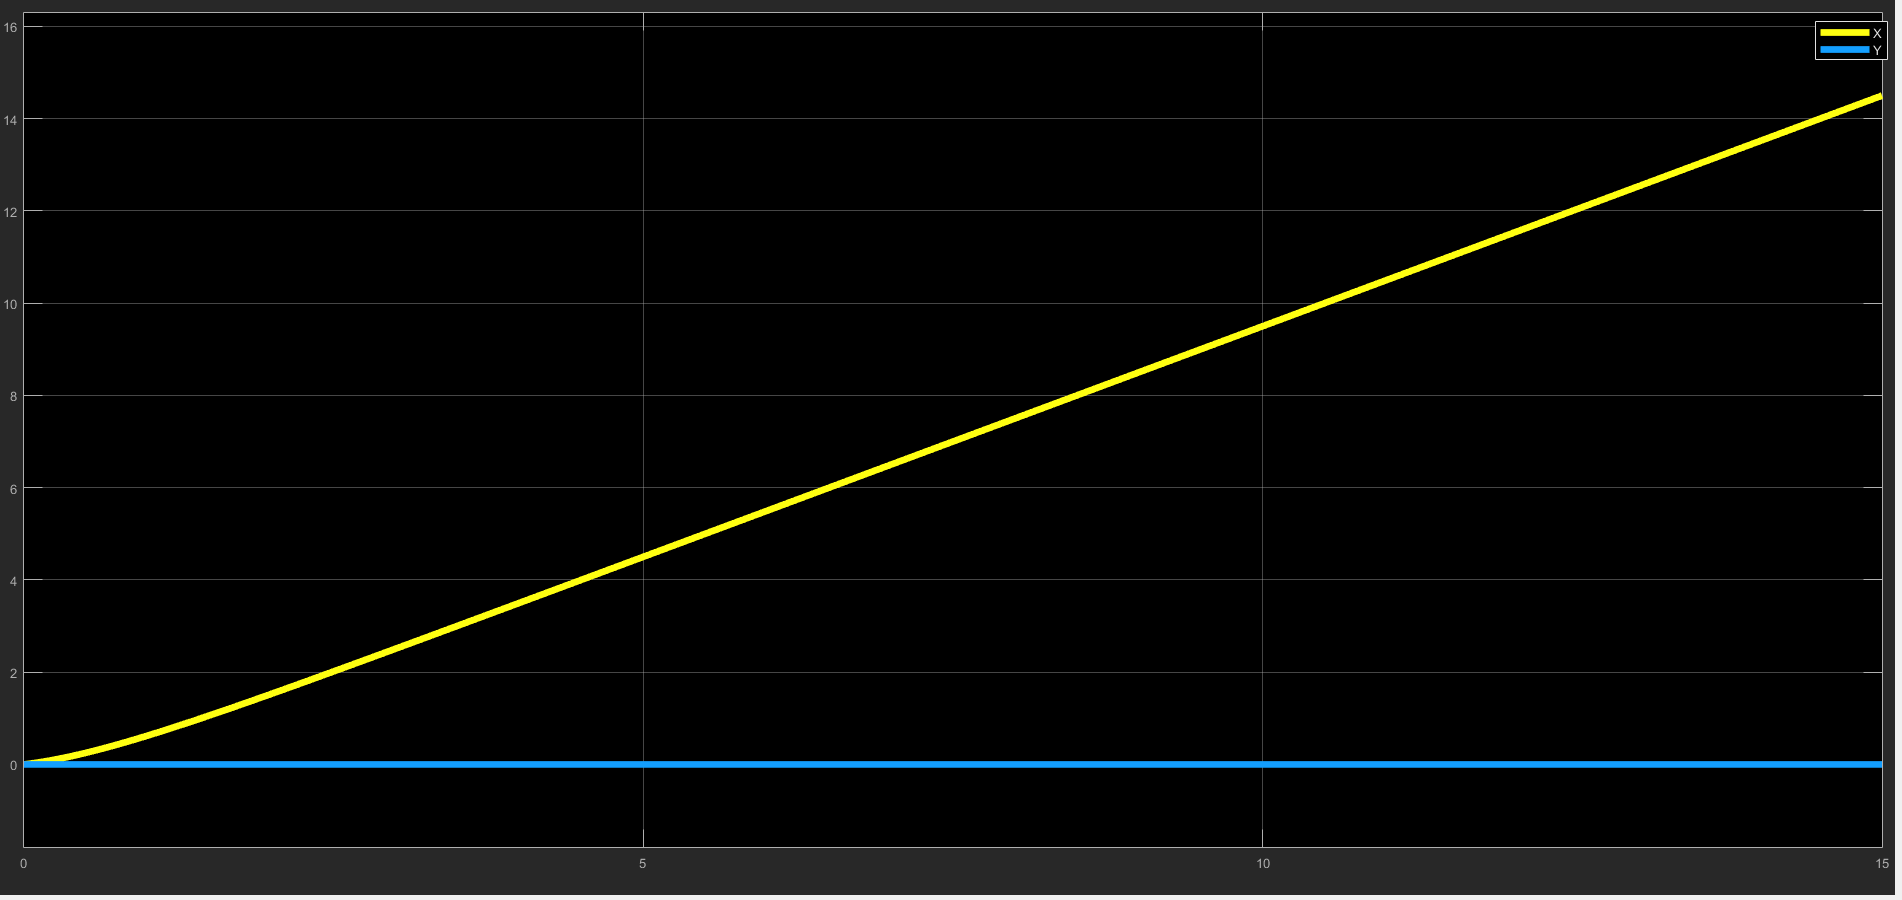
\includegraphics[width=1.0\textwidth]{./img/xy10.PNG}
\caption {\label{fig:sim1 - pos}Car position v=1m/s, teta=0rad}
\end{figure}
As the teta is equal to 0 rad, only 1 coordinate of the car is moving, as the figure \ref{fig:sim1 - pos} demonstrates. The x coordinate is equal to 0 the entire simulation time, and the y coordinate is increasing with a linear scope equal to the linear velocity of the car. This implies that the car is indeed moving in a straight line.\\
\newpage
Changing the teta to 0.1 rad to simulate constant tilt of the smart phone to the right, and maintaining the value of the speed reference in 1 m/s :\
\begin{figure}[!h]
\centering
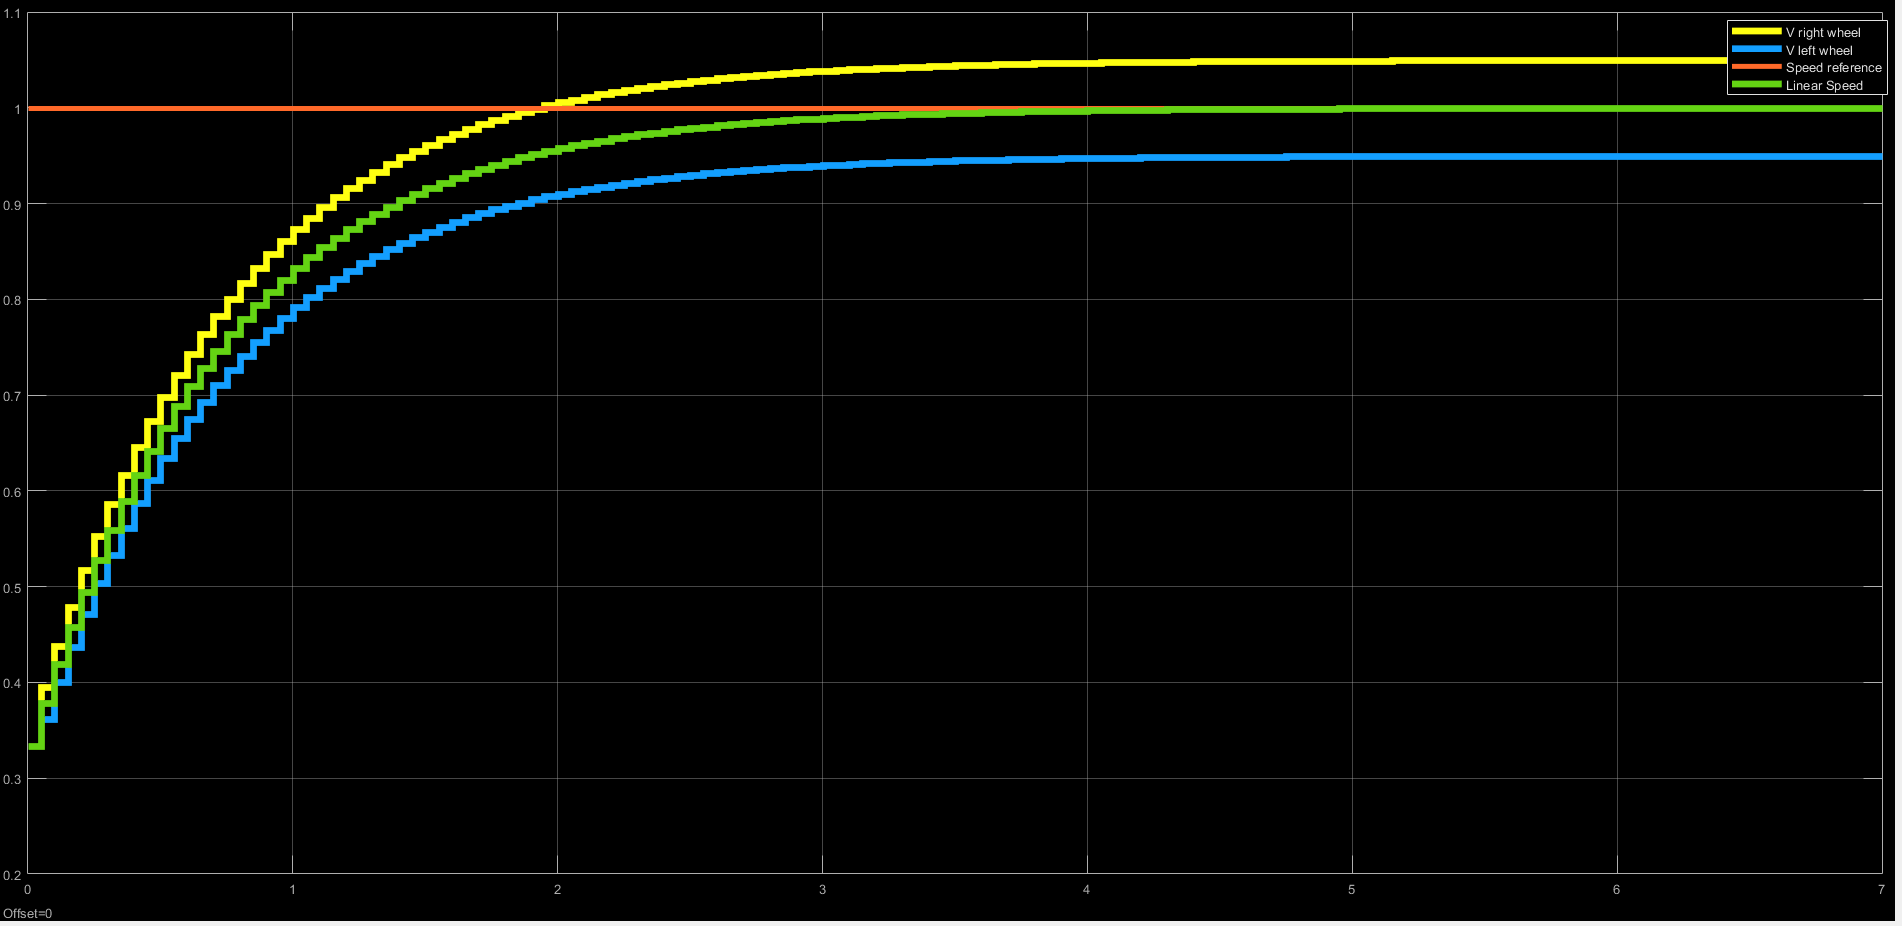
\includegraphics[width=1.0\textwidth]{./img/vel101.PNG}
\caption {\label{fig:sim2 - vel}Linear speed v=1m/s, teta=0.1rad}
\end{figure}
In this simulation it can be observed that having a angle of tilt not equal to 0, causes the left and right wheels to have different velocities, in order to make the car turn. Running more simulations with different values of teta, the outcome shows that the bigger the module of the value of teta, the bigger the difference between the linear velocities of the wheels.
\begin{figure}[!ht]
\centering
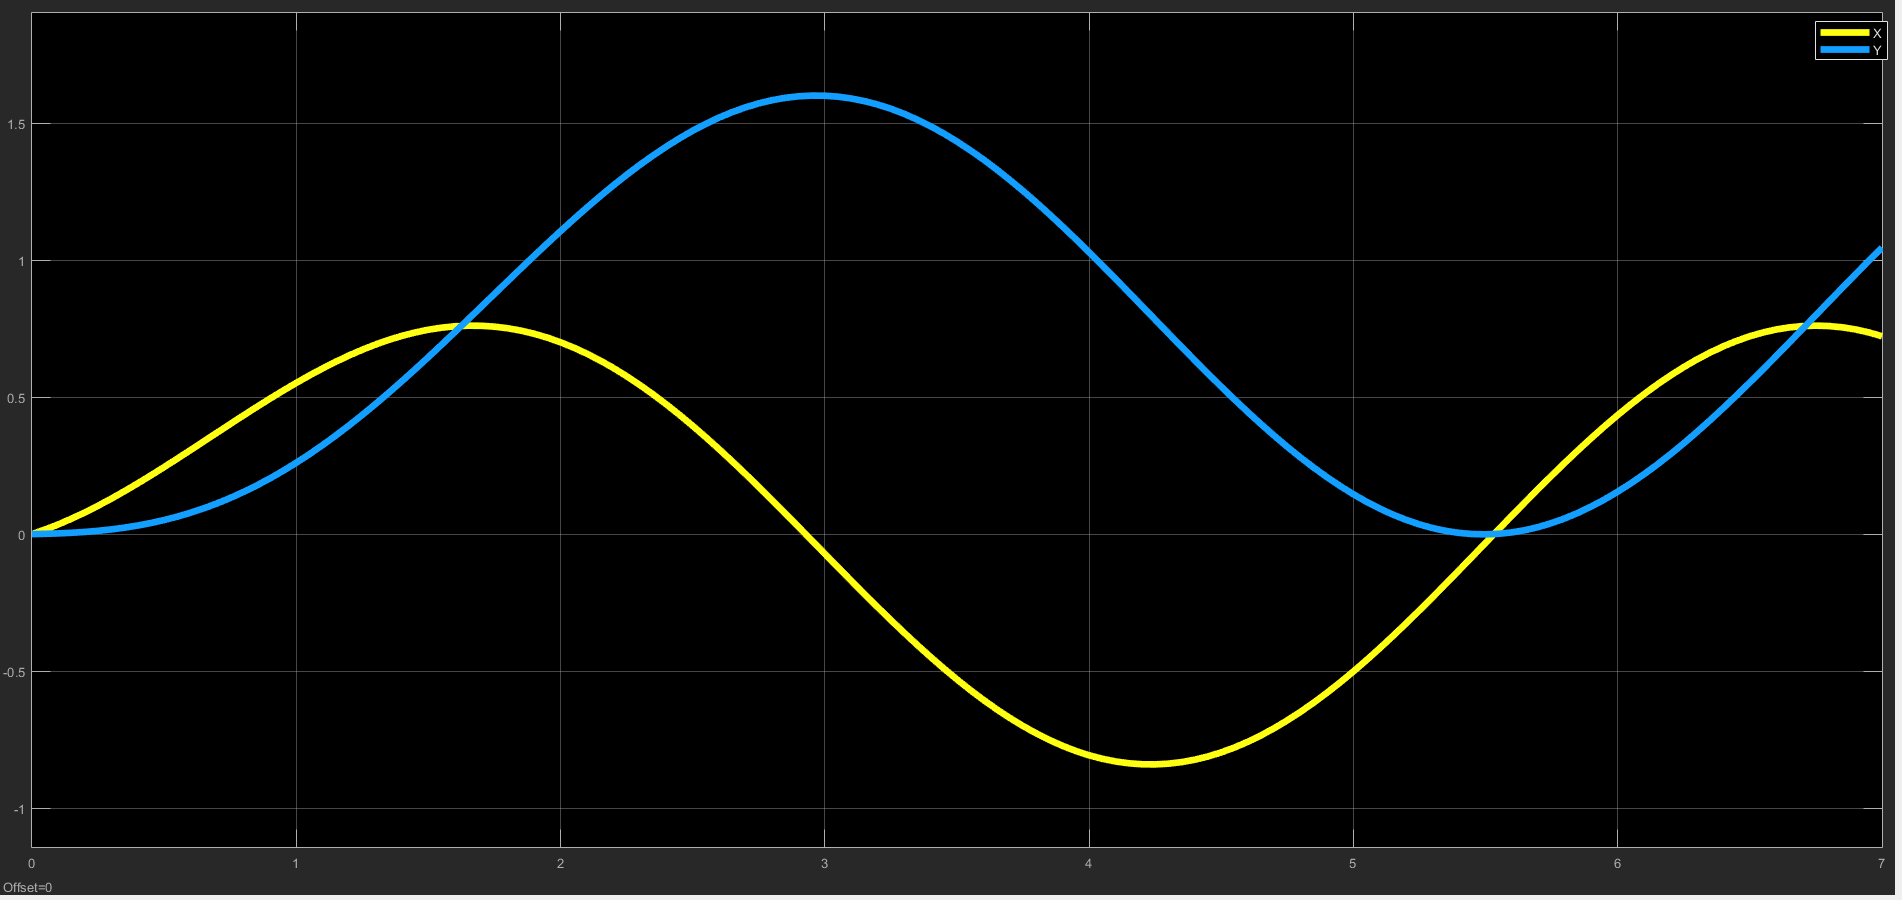
\includegraphics[width=1.0\textwidth]{./img/xy101.PNG}
\caption {\label{fig:sim2 - pos}Linear speed v=1m/s, teta=0.1rad}
\end{figure}
With this figure \ref{fig:sim2 - pos} it is possible to observe that both the position of x and y of the car change with time. With a constant angle of tilt, the car will turn constantly in the same direction, eventually making a 360 degrees turn and as the car as small dimensions, it takes a very small time for it to do so, which is what is observed is this simulation.